\documentclass{beamer}
\mode<presentation>{}
\usepackage{beamerthemesplit}

\usepackage{booktabs}
\usepackage{graphicx}
\usepackage{multimedia}

\newcommand{\set}[1]{\left\{#1\right\}}

\begin{document}

\title[OLIM for Eikonal]{Ordered Line Integral Methods \\
  for Solving the Eikonal Equation}
\author{Sam~Potter \and Maria~Cameron}

\frame{\titlepage}

\begin{frame}
  \frametitle{The eikonal equation} Nonlinear, first-order, hyperbolic
  PDE modeling high frequency wave propagation through inhomogeneous
  media:
  \begin{align*}
    \begin{cases}
      \|\nabla u(x)\| = s(x), & x \in \Omega \\
      \left. u \right|_{D} = 0, & D \subseteq \Omega
    \end{cases}
  \end{align*}
  where:
  \begin{itemize}
  \item $u(x)$ is the first arrival time
  \item $s(x)$ is the slowness or index of refraction
  \item $1/s(x)$ is the speed of propagation
  \end{itemize}
\end{frame}

\begin{frame}
  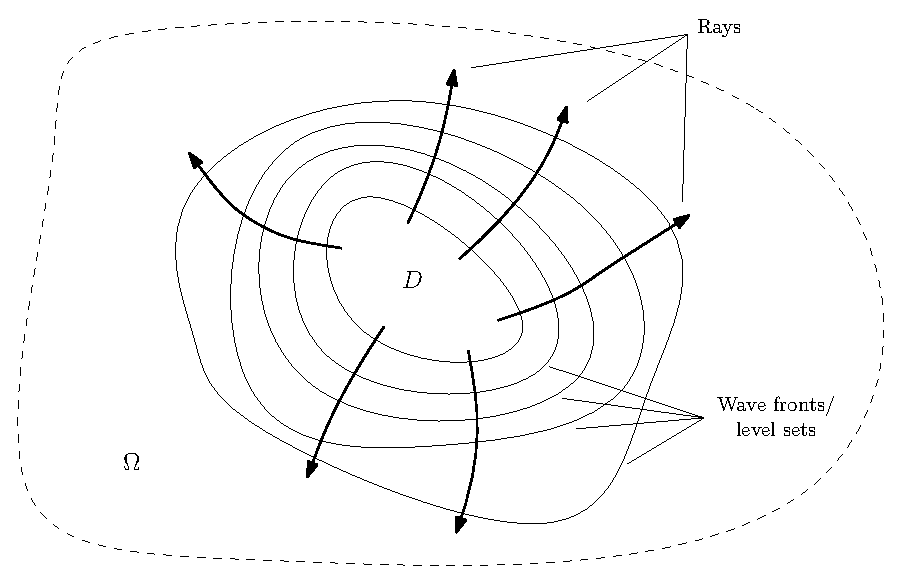
\includegraphics[width=\linewidth]{level-sets.eps}
\end{frame}

\begin{frame}
  \frametitle{Solution methods}
  \begin{itemize}
  \item Ray-tracing: solve ODEs along rays emitted from source\pause
  \item Dijkstra-like: $O(N \log N)$ \pause
    \begin{itemize}
    \item Tsitsiklis 1995\pause
    \item Sethian 1996 (The fast marching method) \pause
    \item \textbf{Our work}\pause
    \end{itemize}
  \item Dial-like: $O(N)$ \pause
  \item Fast sweeping
  \end{itemize}    
\end{frame}

\begin{frame}
  \frametitle{Ordered line integral method (OLIMs)}
  \begin{itemize}
  \item Potter \& Cameron, ``OLIM for Eikonal'', 2018 \pause
  \item Other Cameron: OLIM for quasipotential, recent \pause
  \item Enhancements vs. FMM or Tsitsiklis: \pause
    \begin{itemize}
    \item Quadrature rules \pause
    \item Partitioning neighborhoods \pause
    \item Searching through updates \pause
    \item Update pruning \pause
    \end{itemize}
  \item Some theoretical justification \pause
  \item Use additive local factoring
  \end{itemize}
\end{frame}

\begin{frame}
  \movie[width=\linewidth,height=3in]{}{eikonal.mov}
\end{frame}

\begin{frame}
  \frametitle{Solving the eikonal equation in 2D}
  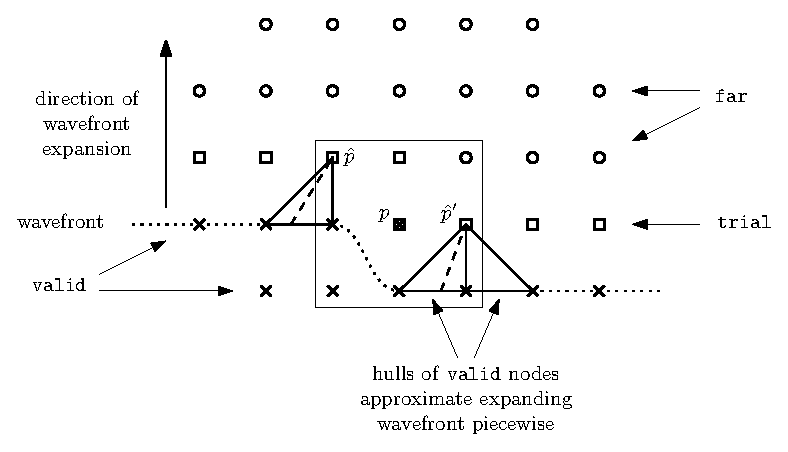
\includegraphics[width=\linewidth]{overview.eps}
\end{frame}

\begin{frame} % explain quadrature rules here and write on board
  \frametitle{Quadrature}
  \begin{tabular}{cc}
    \texttt{rhr}: & right-hand rule \\
    \texttt{mp0}: & simplified midpoint rule \\
    \texttt{mp1}: & midpoint rule
  \end{tabular}
  \begin{center}
    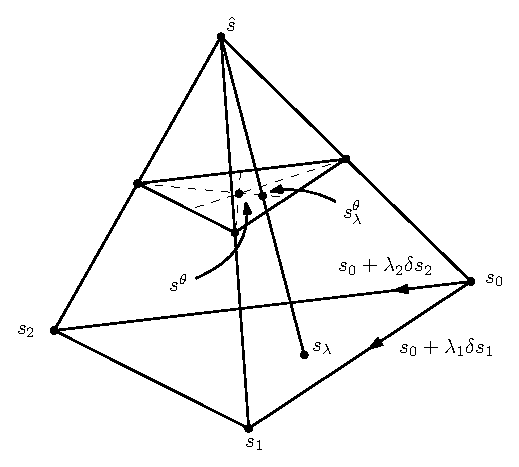
\includegraphics[width=0.7\linewidth]{slowness-tetra.eps}
  \end{center}
\end{frame}

\begin{frame}
  \frametitle{Two family of algorithms}
  \begin{center}
    \begin{tabular}{c|cc}
      & Top-down & Bottom-up \\
      \midrule
      Update choice & Simplex groups & Neighborhood search \\
      Order of updates & High to low & Low to high \\
      Skip updates & Constrained optimization & KKT theory \\
      Solver & SQP & Direct/Newton
    \end{tabular}
  \end{center}
\end{frame}

\begin{frame}
  \frametitle{``Top-down'' hierarchical algorithm}
  \centering
  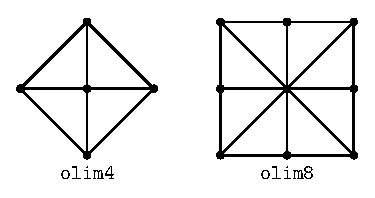
\includegraphics{neighborhood-2d.eps}
  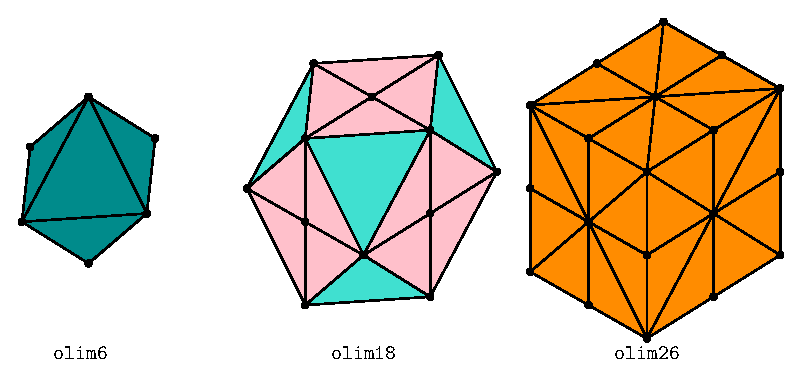
\includegraphics[width=\linewidth]{neighborhood-3d.eps}
\end{frame}

\begin{frame} % fast procedure for enumeration
  \frametitle{``Top-down'' hierarchical algorithm}
  \centering
  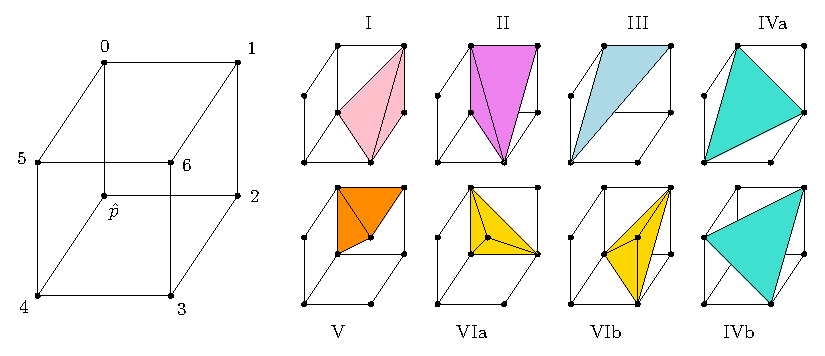
\includegraphics[width=0.65\linewidth]{simplex-groups.eps}
  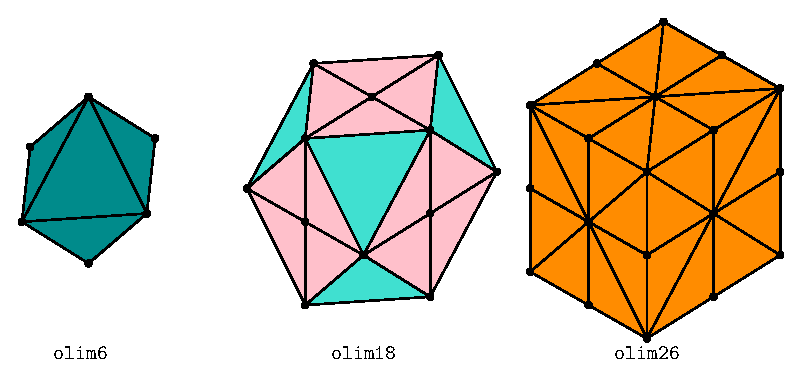
\includegraphics[width=\linewidth]{neighborhood-3d.eps}
\end{frame}

\begin{frame}
  \frametitle{``Top-down'' hierarchical algorithm}
  \centering
  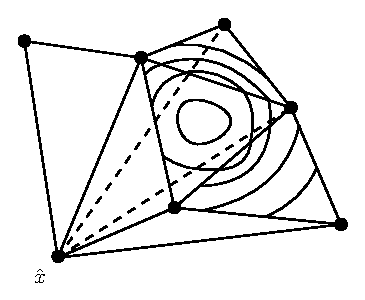
\includegraphics[width=0.75\linewidth]{top-down-algorithm.eps}
\end{frame}

\begin{frame}
  \frametitle{``Top-down'' hierarchical algorithm}
  \centering
  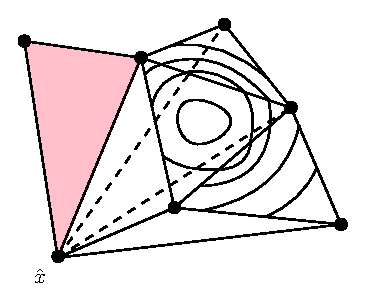
\includegraphics[width=0.75\linewidth]{top-down-algorithm-1.eps}
\end{frame}

\begin{frame}
  \frametitle{``Top-down'' hierarchical algorithm}
  \centering
  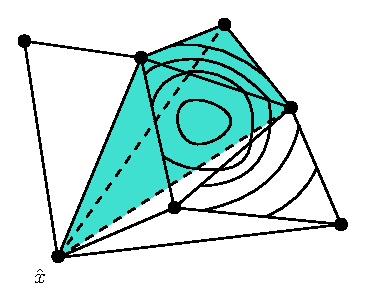
\includegraphics[width=0.75\linewidth]{top-down-algorithm-2.eps}
\end{frame}

\begin{frame}
  \frametitle{``Top-down'' hierarchical algorithm}
  \centering
  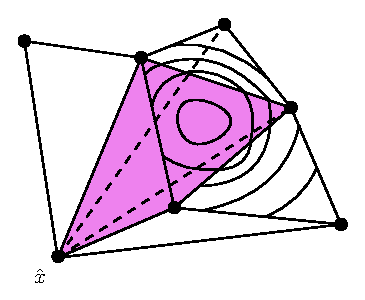
\includegraphics[width=0.75\linewidth]{top-down-algorithm-3.eps}
\end{frame}

\begin{frame}
  \frametitle{``Top-down'' hierarchical algorithm}
  \centering
  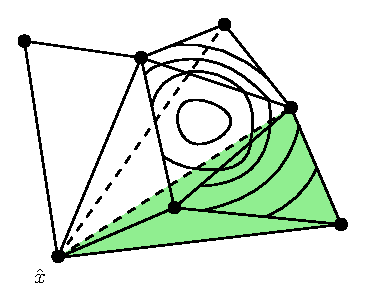
\includegraphics[width=0.75\linewidth]{top-down-algorithm-4.eps}
\end{frame}

\begin{frame}
  \frametitle{``Bottom-up'' hierarchical algorithm}
  \centering
  \vspace{1em}
  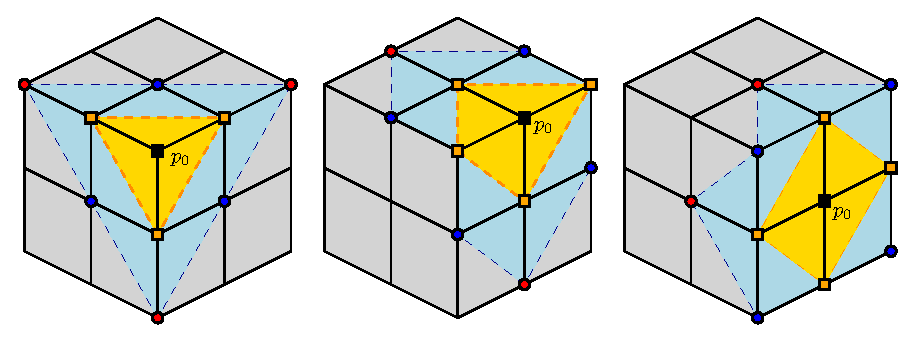
\includegraphics[width=\linewidth]{hu-neighborhoods.eps}
\end{frame}

\begin{frame}
  \frametitle{``Bottom-up'' hierarchical algorithm}
  \centering
  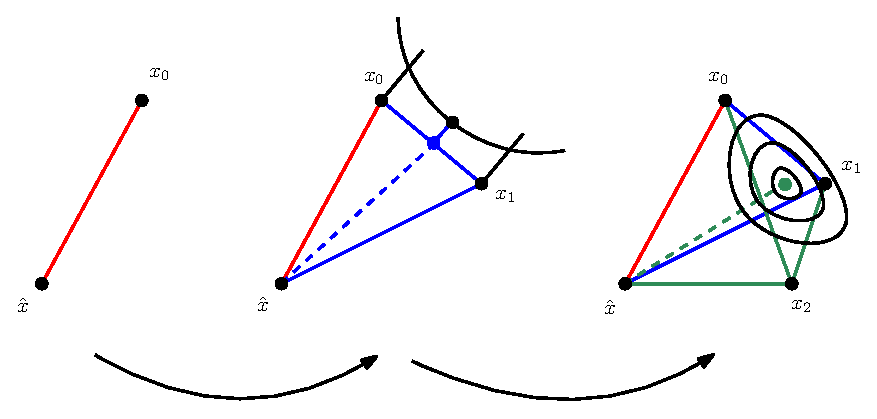
\includegraphics[width=\linewidth]{hierarchical-updates.eps}
\end{frame}

\begin{frame}
  \frametitle{Theoretical results}
  \begin{itemize}
  \item Validation of \texttt{mp0}: $O(h^3)$ error per update \pause
  \item Exact solution for \texttt{rhr} and \texttt{mp0}: QR decomposition \pause
  \item Validation of hierarchical update in 2D\pause:
    \begin{itemize}
    \item Bad nodes don't propagate error \pause
    \item Intuitively: error only occurs when fronts collide
    \end{itemize}
  \end{itemize}
\end{frame}

\begin{frame}
  \frametitle{Additive factoring}
  \begin{itemize}
  \item Point sources and obstacles with corners create singularities
    which lead to $O(h \log \tfrac{1}{h})$ error instead of
    $O(h)$\footnote{Qi \& Vladimirsky, ``Corner cases, singularities,
      and dynamic factoring'', 2018.} \pause
  \item Solve factored eikonal equation to recover $O(h)$ error:
    \begin{align*}
      u = \tau + T
    \end{align*} \pause
  \item Solve for $\tau$, where $T$ is a correction term \pause
  \item Global factoring: solve this equation everywhere
    \begin{itemize}
    \item Exact for $s \equiv 1$
    \end{itemize} \pause
  \item Local factoring: only factor constant-size regions containing singularities
  \end{itemize}
\end{frame}

\begin{frame}
  \frametitle{Local factoring errors ($s \equiv 1$)}
  \centering
  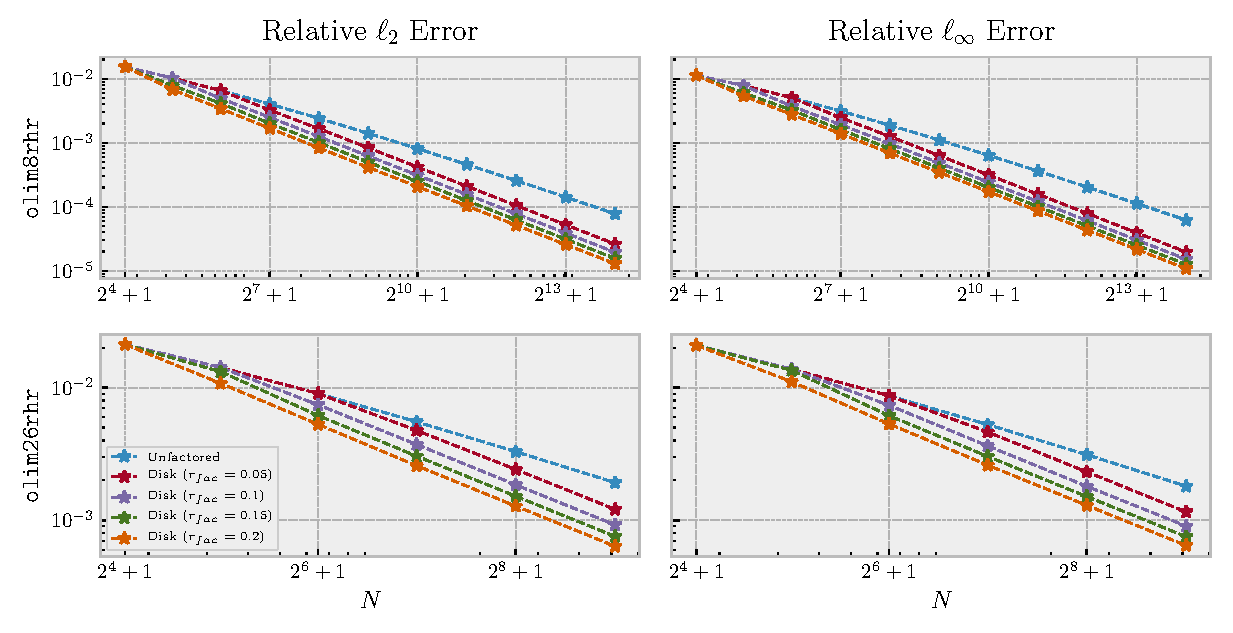
\includegraphics[width=\linewidth]{factoring-error-example.eps}
\end{frame}

\begin{frame}
  \frametitle{Qi \& Vladimirsky's linear speed in 2D}
  Domain: $\Omega = [0, 1]^2$
  \begin{align*}
    \frac{1}{s_i(x)} &= \frac{1}{s_i} + v^\top {(x - x_i)} \\
    u_i(x) &= \frac{1}{\|v\|} \cosh^{-1} \left(1 + \frac{s_i}{2} s(x) \|v\|^2 \|x - x_i\|^2\right) \\
    u(x) &= \min_i u_i(x)
  \end{align*}
  Point sources at $x_1 = (0, 0)$ and $x_2 = (0.8, 0)$
\end{frame}

\begin{frame}
  \frametitle{Qi \& Vladimirsky's linear speed in 2D}
  \centering
  \includegraphics[width=0.9\linewidth]{LF.pdf}
\end{frame}

\begin{frame}
  \frametitle{Single point source with different slowness functions}
  Domain: $\Omega = [-1, 1]^2, [-1, 1]^3$
  \vspace{1em}
  \begin{center}
  \begin{tabular}{cccc}
    Name & $u(x)$ & $s(x)$ \\
    \midrule
    \texttt{s1} & $\cos(r) + r - 1$ & $1 - \sin(r)$ \\
    \texttt{s4} & $\tfrac{1}{2} x^\top A^{1/2} x$, $A$ spd & $\|x\|_A = \sqrt{x^\top A x}$
  \end{tabular}
  \end{center}
\end{frame}

\begin{frame}
  \frametitle{Point source: $s = s_1$, size vs.\ error}
  \centering
  \includegraphics[width=0.75\linewidth]{tmp-pdf/legend.pdf} \\
  \includegraphics[width=0.055\linewidth]{tmp-pdf/s1-y-axis.pdf}
  \includegraphics[width=0.695\linewidth]{tmp-pdf/s1-N-vs-error.pdf} \\
  \includegraphics[width=0.75\linewidth]{tmp-pdf/s1-x-axis.pdf}
\end{frame}

\begin{frame}
  \frametitle{Point source: $s = s_1$, time vs.\ error}
  \centering
  \includegraphics[width=0.75\linewidth]{tmp-pdf/legend.pdf} \\
  \includegraphics[width=0.054\linewidth]{tmp-pdf/s1-y-axis.pdf}
  \includegraphics[width=0.696\linewidth]{tmp-pdf/s1-T-vs-error.pdf} \\
  \hspace{1em}\includegraphics[width=0.66\linewidth]{tmp-pdf/s1-x-axis.pdf}
\end{frame}

\begin{frame}
  \frametitle{Point source: $s = s_4$, size vs.\ error}
  \centering
  \includegraphics[width=0.75\linewidth]{tmp-pdf/legend.pdf} \\
  \includegraphics[width=0.75\linewidth]{tmp-pdf/relative-linf-error.pdf} \\
  \vspace{-1.5em}
  \includegraphics[width=0.065\linewidth]{tmp-pdf/s4-y-axis.pdf}
  \includegraphics[width=0.685\linewidth]{tmp-pdf/s4-N-vs-error.pdf} \\
  \includegraphics[width=0.75\linewidth]{tmp-pdf/s4-x-axis.pdf}
\end{frame}

\begin{frame}
  \frametitle{Point source: $s = s_4$, time vs.\ error}
  \centering
  \includegraphics[width=0.75\linewidth]{tmp-pdf/legend.pdf} \\
  \includegraphics[width=0.75\linewidth]{tmp-pdf/relative-linf-error.pdf} \\
  \vspace{-1.5em}
  \includegraphics[width=0.065\linewidth]{tmp-pdf/s4-y-axis.pdf}
  \includegraphics[width=0.685\linewidth]{tmp-pdf/s4-T-vs-error.pdf} \\
  \hspace{1.1em}\includegraphics[width=0.64\linewidth]{tmp-pdf/s4-x-axis.pdf}
\end{frame}

\begin{frame}
  \frametitle{Conclusion}
  Our contributions:\pause
  \begin{itemize}
  \item Fast and accurate eikonal solver\pause:
  \item Improvement over fast marching method in many cases \pause
  \item Developed algorithmic techniques which are generally useful \pause
  \end{itemize}
  Benefits for HF wave propagation problems\pause:
  \begin{itemize}
  \item Improved directional coverage $\implies$ high accuracy solvers \pause
  \item Easy recovery of characteristics \pause
  \item Multiple arrivals \pause
  \item Dynamic local factoring
  \end{itemize}
\end{frame}

\end{document}

%%% Local Variables:
%%% mode: latex
%%% TeX-master: t
%%% End:
